\section{Parameter model}
\label{sec:parameterModel}
\label{maths:parameter_defn}
\label{maths:parameter-model}

The following section outlines the parameter model. We consider three types of parameter model:
\begin{itemize}
\item
Type 1. Equation type
\begin{align*}
\psi_i = H(\beta, C_i, \eta_i)
\end{align*}
This is the most general form of a parameter model with no constraints on the function $H$.
It is an implicit equation as it doesn't allow an easy interpretation of its elements in contrast to the two following forms.
\item
Type 2. Gaussian model with general covariate model
\begin{align*}
h(\psi_i) = H(\beta, C_i) + \eta_i
\end{align*}
Here the parameter is normally distributed up to a transformation $h$ with a general covariate model and additive random effects.
\item
Type 3. Gaussian model with linear covariate model
\begin{align*}
h(\psi_i) = h(\psi_{pop}) + \beta \, C_i + \eta_i
\end{align*}
This is a special case of the models above which allows for the most detailed interpretation as explained in the following section.
\end{itemize}
with
\begin{itemize}
\item
$\psi_i$ -- individual parameter
\item
$\psi_{pop}$ -- typical or population mean parameter
\item
$\eta_i$ -- random effect(s)
\item
$\beta$ -- fixed effect(s)
\item
$C_i$ -- covariate(s)
\item
H -- arbitrary function
\item
h -- function which transforms the model on both sides, e.g. log, logit, probit.
\end{itemize}

\subsection{Discussion and examples of Type 1 models}
\label{subsec:paramModelType1}
This model type is the most flexible one, able to accommodate
\begin{itemize}
\item
multiple fixed effects
\item
multiple random effects and
\item
an arbitrary (nonlinear) covariate model.
\end{itemize}

\paragraph{Example}
Let's consider a complex clearance model as introduced in \cite{NONMEM:2006aa}, which contains
\begin{itemize}
\item
four fixed effects $\theta_1, \cdots, \theta_4$
\item
three continuous covariates $WT, AGE, SECR$
\item
one categorical covariate $ICU$
\item
three random effects $\eta_{1i,met}\sim \mathcal{N}(0,\omega_{1,met}^2),\eta_{2i,met}\sim \mathcal{N}(0,\omega_{2,met}^2), \eta_{3i,ren}\sim \mathcal{N}(0,\omega_{3,ren}^2)$
\end{itemize}
The model is composed of
\begin{enumerate}
\item
the average metabolic clearance which reads
\begin{align*}
& CL_{met_{average}} = WT\times \frac{\theta_1 - \theta_2 \times Cpss_2}{\theta_3 + Cpss_2}
\end{align*}
extended with random effects representing a patient being from an ICU (intensive care unit) or else
\begin{align*}
& CL_{i,met} = CL_{met_{average}} + (1 - ICU) \; \eta_{1,i} + ICU \; \eta_{2,i}
\end{align*}
i.e.
\begin{align*}
& CL_{i,met} = \left\{ \begin{array}{lcl}  CL_{met_{average}} + \eta_{1,i}  & \mbox{for} & ICU = 0 \quad \text{i.e. patient not from ICU} \\
CL_{met_{average}} + \eta_{2,i}  & \mbox{for} & ICU = 1 \quad \text{else}
\end{array}\right.
\end{align*}
\item
and average renal clearance which reads
\begin{align*}
& CL_{ren_{average}} = \theta_4 \times RF \quad \text{with}  \quad
RF = WT\times \frac{1.66 - 0.011 \times AGE}{SECR}
\end{align*}
so the clearance for subject $i$ amounts to
\begin{align*}
& CL_{i,ren} = CL_{ren_{average}}(1+ \eta_{3,i})
\end{align*}
\end{enumerate}
The complete model, combining (1) and (2), for an individual's clearance then reads
\begin{align*}
& CL_i = CL_{i,met} + CL_{i,ren}.
\end{align*}
This model, although fully flexible, is difficult to break into meaningful sub-components. This is an entirely different situation for the following model types, where clearly defined sub-components can be separately stored and annotated.
%\begin{itemize}
%\item
%metabolic clearance
%\begin{align*}
%& CL_{met_{average}} = WT\times \frac{\theta_1 - \theta_2 \times Cpss_2}{\theta_3 + Cpss_2}
%\end{align*}
%extended with random effects representing a patient being from an ICU (Intensive Care Unit) or else
%\begin{align*}
%& CL_{met} = CL_{met_{average}} + (1 - ICU) \, \eta_{1i,met} + ICU \, \eta_{2i,met}
%\end{align*}
%i.e.
%\begin{align*}
%& CL_{met} = \left\{ \begin{array}{lcl}  CL_{met_{average}} + \eta_1  & \mbox{for} & ICU = 0 \quad \text{i.e. patient not from ICU} \\
%CL_{met_{average}} + \eta_2  & \mbox{for} & ICU = 1 \quad \text{else}
%\end{array}\right.
%\end{align*}
%\item
%and renal clearance
%\begin{align*}
% CL_{ren} = \theta_4 \times RF
%\end{align*}
%with
%\begin{align*}
%& RF = WT\times \frac{1.66 - 0.011 \times AGE}{SECR}
%\end{align*}
%with covariates \var{WT}, \var{AGE} and \var{SECR}.
%\end{itemize}
%The complete model for an individual's clearance reads
%\begin{align*}
%& CL_i = CL_{met} + CL_{ren}\; \eta_{3i,ren}.
%\end{align*}

\subsection{Discussion and examples of Type 2 models}
\label{subsec:paramModelType2}
Here, we consider normally distributed parameters, up to a transformation $h$, i.e. normal, log-normal or logit-normally distributed with identity, the natural logarithm or the logit as transformation, respectively.

Compared to the Type 1 parameter model, the Type 2 parameter model has a more structured additive form:
\begin{align*}
h(\psi_i) =
\underbrace{H(\beta, C_i)}_{\text{\parbox{2.5cm}{\centering non-linear covariate\\[-4pt] model}}}
+ \underbrace{\eta_i^{(0)}+ \eta_{ik}^{(+1)} + \dots}_{\text{\parbox{3cm}{\centering IIV and other\\[-4pt] levels of variability}}}
\end{align*}
Accordingly a model for an individual parameter consists of
\begin{itemize}
\item
the left-hand transformation, $h$
\item
a non-linear covariate model, i.e. any function, $H$, of fixed effects, $\beta$, and categorical or continuous covariates, $C_i$, e.g. \textit{Sex} or \textit{Weight}, and
\item
random effects, $\eta$, for \textit{inter-individual, inter-occasion} and/or other levels of variability (see section \ref{sec:variabilityModel}).
\end{itemize}

\paragraph{Example}
The following example is taken from the 'Fisher/Shafer NONMEM Workshop', and in NMTRAN code reads
%\begin{xmlcode}
%	WTE = THETA(1) * WT / (THETA(2)+ WT)
%	V = (THETA(3) + WTE) * EXP(ETA(1))
%\end{xmlcode}
\lstset{language=NONMEMdataSet}
\begin{lstlisting}
	WTE = THETA(1) * WT / (THETA(2)+ WT)
	V = (THETA(3) + WTE) * EXP(ETA(1))
\end{lstlisting}

After taking the logarithm of both sides we get
\begin{align*}
\log(V_i) = \log\Big(\theta_3 + \frac{\theta_1 \times WT_i}{\theta_2 + WT_i}\Big) + \eta_{V,i}.
\end{align*}

\subsection{Discussion and examples of Type 3 models}
\label{subsec:paramModelType3}
Here, we again consider normally distributed parameters, up to a transformation $h$, i.e. normal, log-normal or logit-normally distributed with identity, the natural logarithm or the logit as transformation, respectively.

The Type 3 parameter model has a very convenient fully additive form, which separates all of the sub-components, making it very easy to understand and process:
\begin{align*}
h(X_i) = h(X_{pop})
+ \underbrace{\beta \,C_i}_{\text{\parbox{2cm}{\centering linear covariate\\[-4pt] model}}}
+ \underbrace{\eta_i^{(0)}+ \eta_{ik}^{(+1)} + \dots}_{\text{\parbox{3cm}{\centering IIV and other\\[-4pt] levels of variability}}}
\end{align*}
Accordingly a model for an individual parameter consists of
\begin{itemize}
\item
a parameter transformation, $h$
\item
a typical or population mean value of the parameter, $X_{pop}$
\item
a linear covariate model, $\beta \, C_i$, with
\begin{itemize}
\item
fixed effects, $\beta$, and
\item
categorical or continuous covariates, $C_i$, e.g. \textit{Sex} or \textit{Weight}
\end{itemize}
\item
random effects, $\eta$, for \textit{inter-individual, inter-occasion} and/or other levels of variability (section \ref{sec:variabilityModel}).
\end{itemize}
See Figure \ref{fig:weightAsCovariate} for an example of the linear relationship between a parameter and a continuous covariate and one, \textit{inter-individual}, level of variability.

\paragraph{Example}
Let's consider volume, $V$, as a log-normally distributed parameter with two covariates \textit{Sex} and \textit{Weight} and with three levels of variability as discussed in Example 3 in section \ref{sec:variabilityModel} (see Figure \ref{tree_IOV1}), which can be represented by the equation:
%\begin{align*}
%& \eta_i \sim \mathcal{N}(0,\omega_V); \quad \log( V_i ) = \log( V_{pop} ) + \beta_{V,1} 1_{Sex_i=F} + \beta_{V,2} \log\Big(\frac{W_i}{70}\Big) + \eta_{i,V}
%\end{align*}
\begin{align*}
V_{lik} = V_{pop} e^{\beta_{V,1} 1_{Sex_i=F}} \Big(\frac{W_i}{70}\Big)^{\beta_{V,2}} e^{\eta_{l,V}^{(-1)}}  e^{\eta_{li,V}^{(0)}} e^{\eta_{lik,V}^{(+1)}}
\end{align*}
or alternatively as
\begin{align*}
\underbrace{\log(V_{lik})}_{\text{\parbox{2cm}{\centering transformed\\[-4pt] individual value}}} =
\underbrace{\log(V_{pop})}_{\text{\parbox{2cm}{\centering transformed\\[-4pt] typical value}}} +
\underbrace{\beta_{V,1} 1_{Sex_i=F}}_{\text{\parbox{2.2cm}{\centering categorical\\[-4pt] covariate model\\[-4pt] for Sex}}}
+ \underbrace{\beta_{V,2} \log\Big(\frac{W_i}{70}\Big)}_{\text{\parbox{2.2cm}{\centering continuous\\[-4pt] covariate model\\[-4pt] for Weight}}}
+ \underbrace{\eta_{l,V}^{(-1)}}_{\text{\parbox{1.8cm}{\centering inter-centre\\[-4pt]  variability}}}
+ \underbrace{\eta_{li,V}^{(0)}}_{\text{\parbox{1.8cm}{\centering inter-individual\\[-4pt] within centre \\[-4pt]  variability}}}
+ \underbrace{\eta_{lik,V}^{(+1)}}_{\text{\parbox{2.2cm}{\centering inter-occasion\\[-4pt] within individual \\[-4pt] within centre \\[-4pt] variability}}}
\end{align*}
with
\begin{align*}
 && \eta_{l,V}^{(-1)} \sim \mathcal{N}\big(0,\Omega^{(-1)}\big), \quad \eta_{li,V}^{(0)} \sim \mathcal{N}\big(0,\Omega^{(0)}\big),
\quad \eta_{lik,V}^{(+1)} \sim \mathcal{N}\big(0,\Omega^{(+1)}\big).
\end{align*}
The equation for $V_{lik}$ represented in the additive form is clearly easier to understand and one can read out the following information from it:
\begin{itemize}
\item
the parameter transformation, the natural logarithm, $log$
\item
the typical volume, $V_{pop}$
\item
the two linear covariate models, $\beta_{V,1} C_1$ and $\beta_{V,2} C_2$ with
\begin{itemize}
\item
a fixed effect for the categorical covariate, $\beta_{V,1}$
\item
a categorical covariate, $1_{Sex_i=F}$
\item
a fixed effect for the continuous covariate, $\beta_{V,2}$
\item
a continuous covariate, $C_2 = \log(W/W_{pop})$ with $W_{pop}=70$
\end{itemize}
\item
multiple random effects
\begin{itemize}
\item
a random effect above the subject level for \textit{inter-centre} variability, $\eta_{l,V}^{(-1)}$
\item
a random effect at the subject level for \textit{inter-individual within centre} variability, $\eta_{li,V}^{(0)}$
\item
a random effect below the subject level for \textit{inter-occasion within individual within centre} variability, $\eta_{lik,V}^{(+1)}$.
\end{itemize}
\end{itemize}


\begin{figure}[htbp]
\centering
 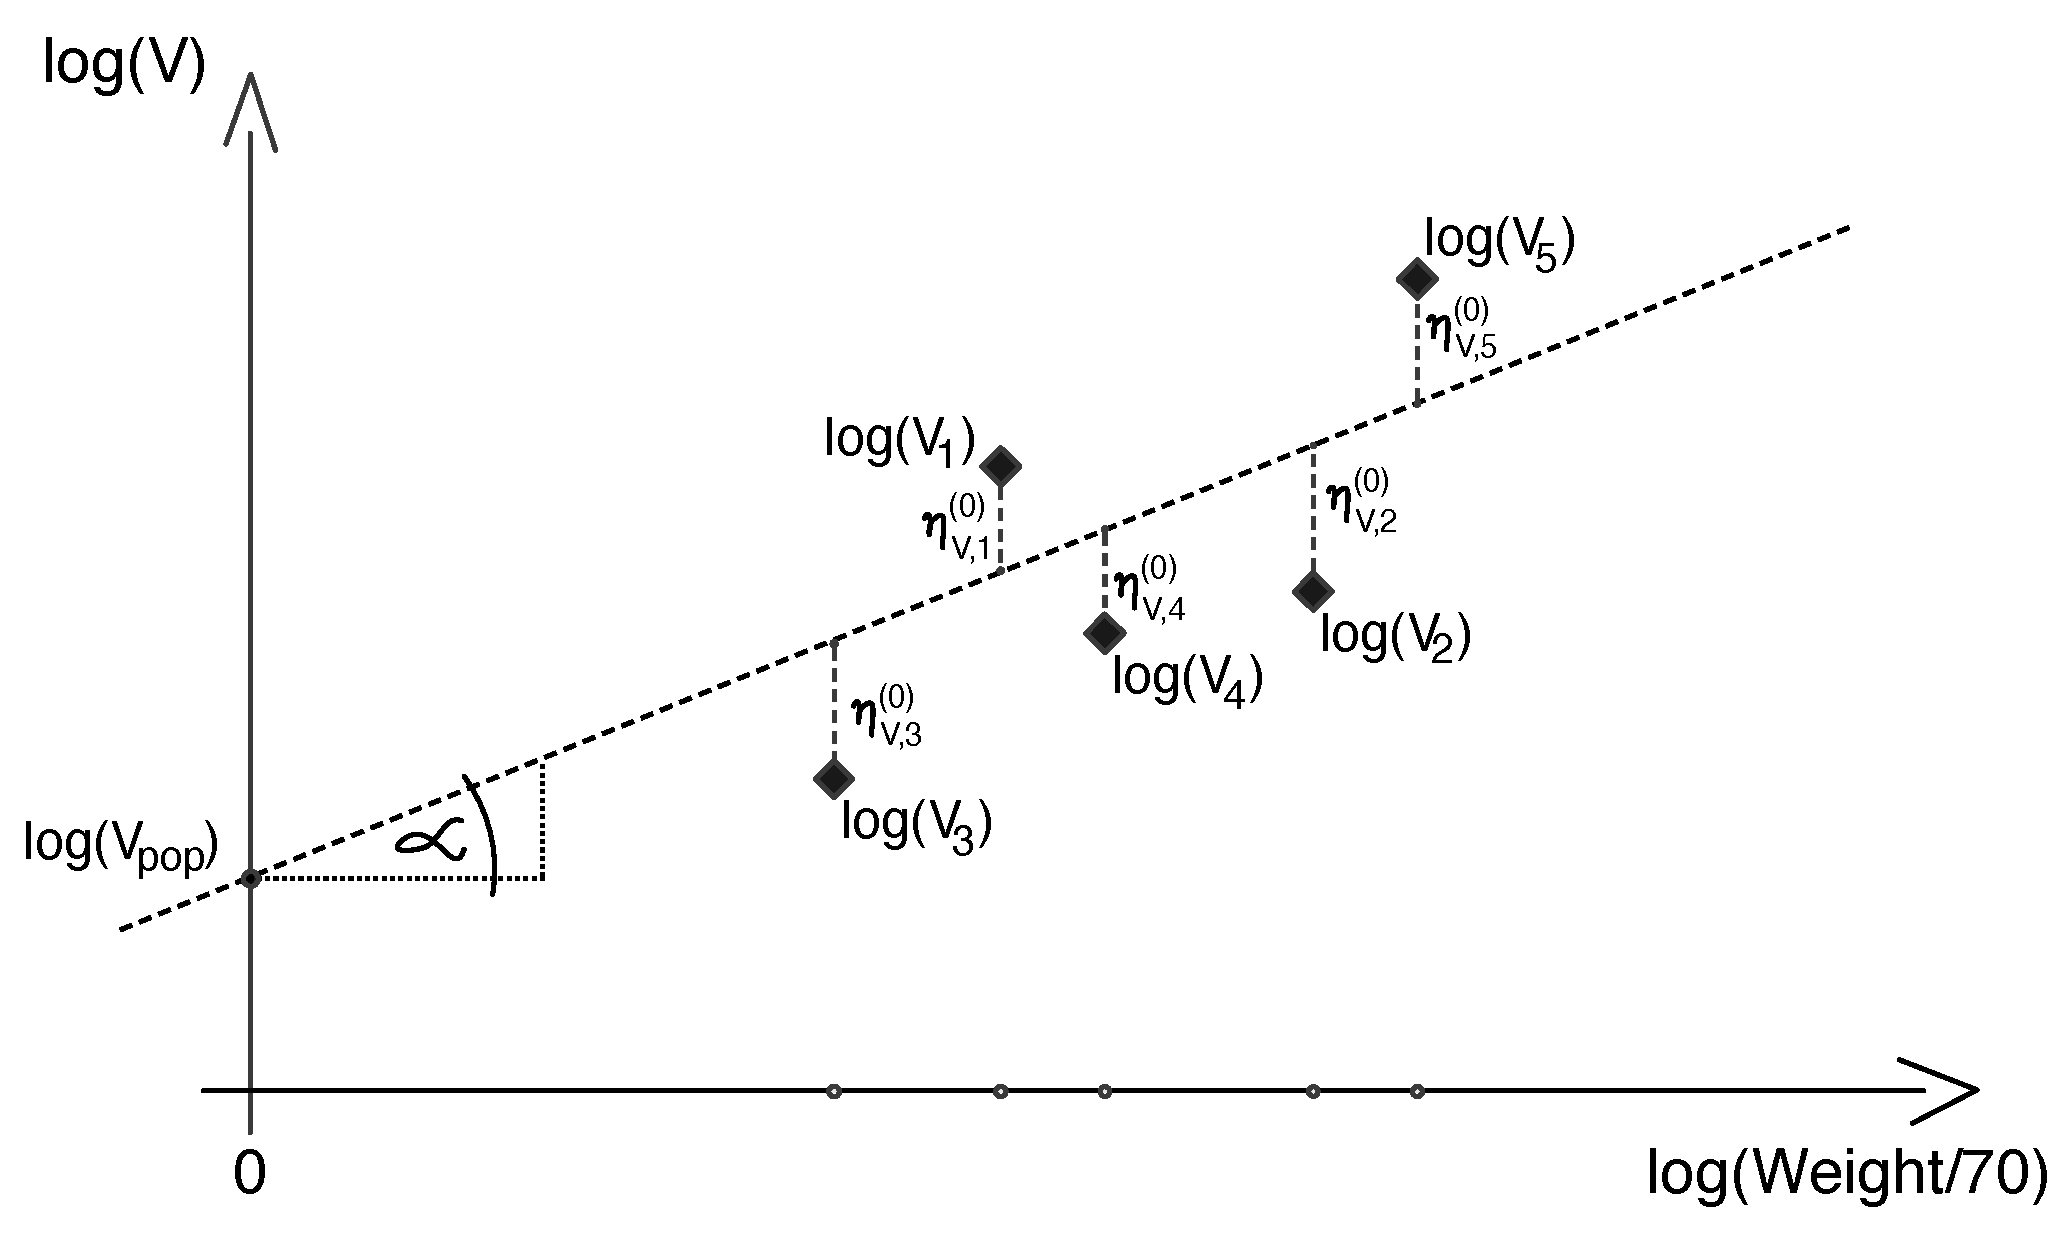
\includegraphics[width=100mm]{pics/weightAsCovariate.pdf}
\caption{The linear relationship between the parameter and a continuous covariate after application of appropriate transformations $V_i \longrightarrow \log(V_i)$ and $W \longrightarrow \log(W/70)$ with $\beta_{V,2} = \tan{\alpha}$, the slope of the regression line, and $\log(V_{pop})$ as the $y$-axis intercept.}
\label{fig:weightAsCovariate}
\end{figure}

%%%%%%%%%%%%%%%%%%%%%%%%%%%%%%%%%%%%%%%%%%%%%%%%%%%%%%%%%%%%%%%%%
\subsection{Correlation of random effects}
\label{subsec:correlationModel}\label{maths:param correlation}
Correlation of random effects means that the transformed parameters. e.g. $\log(V_i)$ and $\log(CL_i)$ are correlated as well (although the relationship is not straightforward; see also the discussion below on correlation and covariates). There are two alternative ways to define the correlation, using either
\begin{itemize}
\item
a correlation matrix, $R$, or
\item
a variance-covariance matrix, $\Omega$.
\end{itemize}


\paragraph{Correlation matrix}
In this case it is sufficient to define the non-zero correlation coefficients, e.g. $\rho_{V,CL}$. All other off-diagonal correlation coefficients will be assumed to be equal to 0. For a simple one-compartment oral PK model with parameters $ka$, $V$, $CL$, and a correlation between $CL$ and $V$ the full correlation matrix reads as follows
\[
R =
 \begin{pmatrix}
  1 	& 0 	& 0  	\\
   		& 1	& \rho_{V,CL} \\
  		& 	& 1
 \end{pmatrix}
\]

\paragraph{Variance-covariance matrix}
\label{maths:covariance-mat-derivation}
Alternatively, the variance-covariance matrix for the model
\[
 \Omega =
 \begin{pmatrix}
  \omega_{ka}^2 	& \omega_{ka,V}	& \omega_{ka,CL}\\
   			  	& \omega_{V}^2	& \omega_{V,CL} \\
  				& 				& \omega_{CL}^2
 \end{pmatrix}
 =
  \begin{pmatrix}
  \omega_{ka}^2 	& 0				& 0 \\
   			  	& \omega_{V}^2	& \omega_{V,CL} \\
  				& 				& \omega_{CL}^2
 \end{pmatrix}
\]
is providing the necessary information due to the reletionship
\begin{align*}
	&\mbox{Cov($p_i$,$p_j$)} = \sigma_i \sigma_j \mbox{Corr($p_i$,$p_j$)}  = \sigma_i \sigma_j \;\rho_{i,j} \quad \mbox{i.e.} \quad \omega_{V,CL} = \omega_V \omega_{CL} \rho_{V,CL}
\end{align*}
in which case it is enough to define $\Omega$ to cover the full correlation structure.

%%%%%%%%%%%%%%%%%%%%%%%%%%%%%%%%%%%%%%%%%%%%%%%%%%%%%%%%%%%%%%%%%
\subsection{Covariate model}
\label{maths:covariate_model}

The covariate model accounts for systematic or known subject
characteristics such as treatment group, gender or body
weight. Accordingly, the model can be defined for discrete and
continuous covariates and is the place where one category of fixed
effects is defined (the other being
the population averages, e.g. $V_{pop}$). Of course, the values of
individual characteristics (weight or sex) are subject specific but
the parameters assigned to them are identical for a group or
population.

As described in the example above the contribution of the continuous
covariate $Weight$ to the parameter value is formulated as
$\beta_{V,2} \log(W_i/70)$ (see figure
\ref{fig:weightAsCovariate}). The figure illustrates the linearity
after the appropriate transformation of the parameter, $V_i
\longrightarrow \log(V_i)$ and $W \longrightarrow \log(W/70)$ with
$\beta_{V,2} = \tan{\alpha}$, the slope of the regression line, and
$\log(V_{pop})$ as the $y$-axis intercept.

In the estimation case the values for the covariate are provided for
each individual. In the case of a simulation (see example
\ref{subsec:exp2_TaskDescription}) its probability distribution has to
be estimated. The information we have to provide is summarised in the
following
\paragraph{Continuous covariate model}
\begin{align*}
Covariates & =  Weight  \\
CovariatesType & = Continuous  \\
CovariatesPopDistribution\{1\} & \sim \mbox{Normal}(pop_{Weight}, \omega_{Weight})  \\
 \text{with} & \quad pop_{Weight}=70.07 \\
 & \quad \omega_{Weight}=14.09  \\
CovariatesTransf & =\log(Weight/70) 
\end{align*}
Analog information has to be provided in the case of a categorical covariate, 
such as \textit{Sex} and is summarised for a simple example in the following

\paragraph{Categorial covariate model}
\begin{align*}
Covariates &= Sex   \\
CovariatesType &= Categorical  \\
CategoriesNumber &= 2   \\
Categories &= \{F,M\}   \\
RefCategory &= F   \\
RefCategProbability &= 14/36 
\end{align*}


%%%%%%%%%%%%%%%%%%%%%%%%%%%%%%%%%%%%%%%%%%%%%%%%%%%%%%%%%%%%%%%%%%%
%%\subsection{Note on correlation and covariates}
%%This section discusses the influence of covariates on correlation between random effects and that of the parameters. In the case without e.g. normally distributed covariates, the correlation is identical. However, the presence of normally distributed body weight in the parameter model has interesting consequences for these correlations. \\
%%Let's consider as an example two correlated log-normally distributed parameters, $V$ and $CL$, without covariates i.e.
%%\begin{align*}
%%& \eta_{V} \sim \mathcal{N}(0,\omega_V); \quad \log( V ) = \log( V_{pop} ) + \eta_{V}  \\
%%& \eta_{CL} \sim \mathcal{N}(0,\omega_{CL}); \quad \log( CL ) = \log( CL_{pop} ) + \eta_{CL}
%%\end{align*}
%%then the correlation between the random effects is identical to the correlation of the (transformed) parameters, see Figure \ref{fig:correlationEtasLogedParams1}.
%%\begin{figure}[h!]
%%\centering
%% 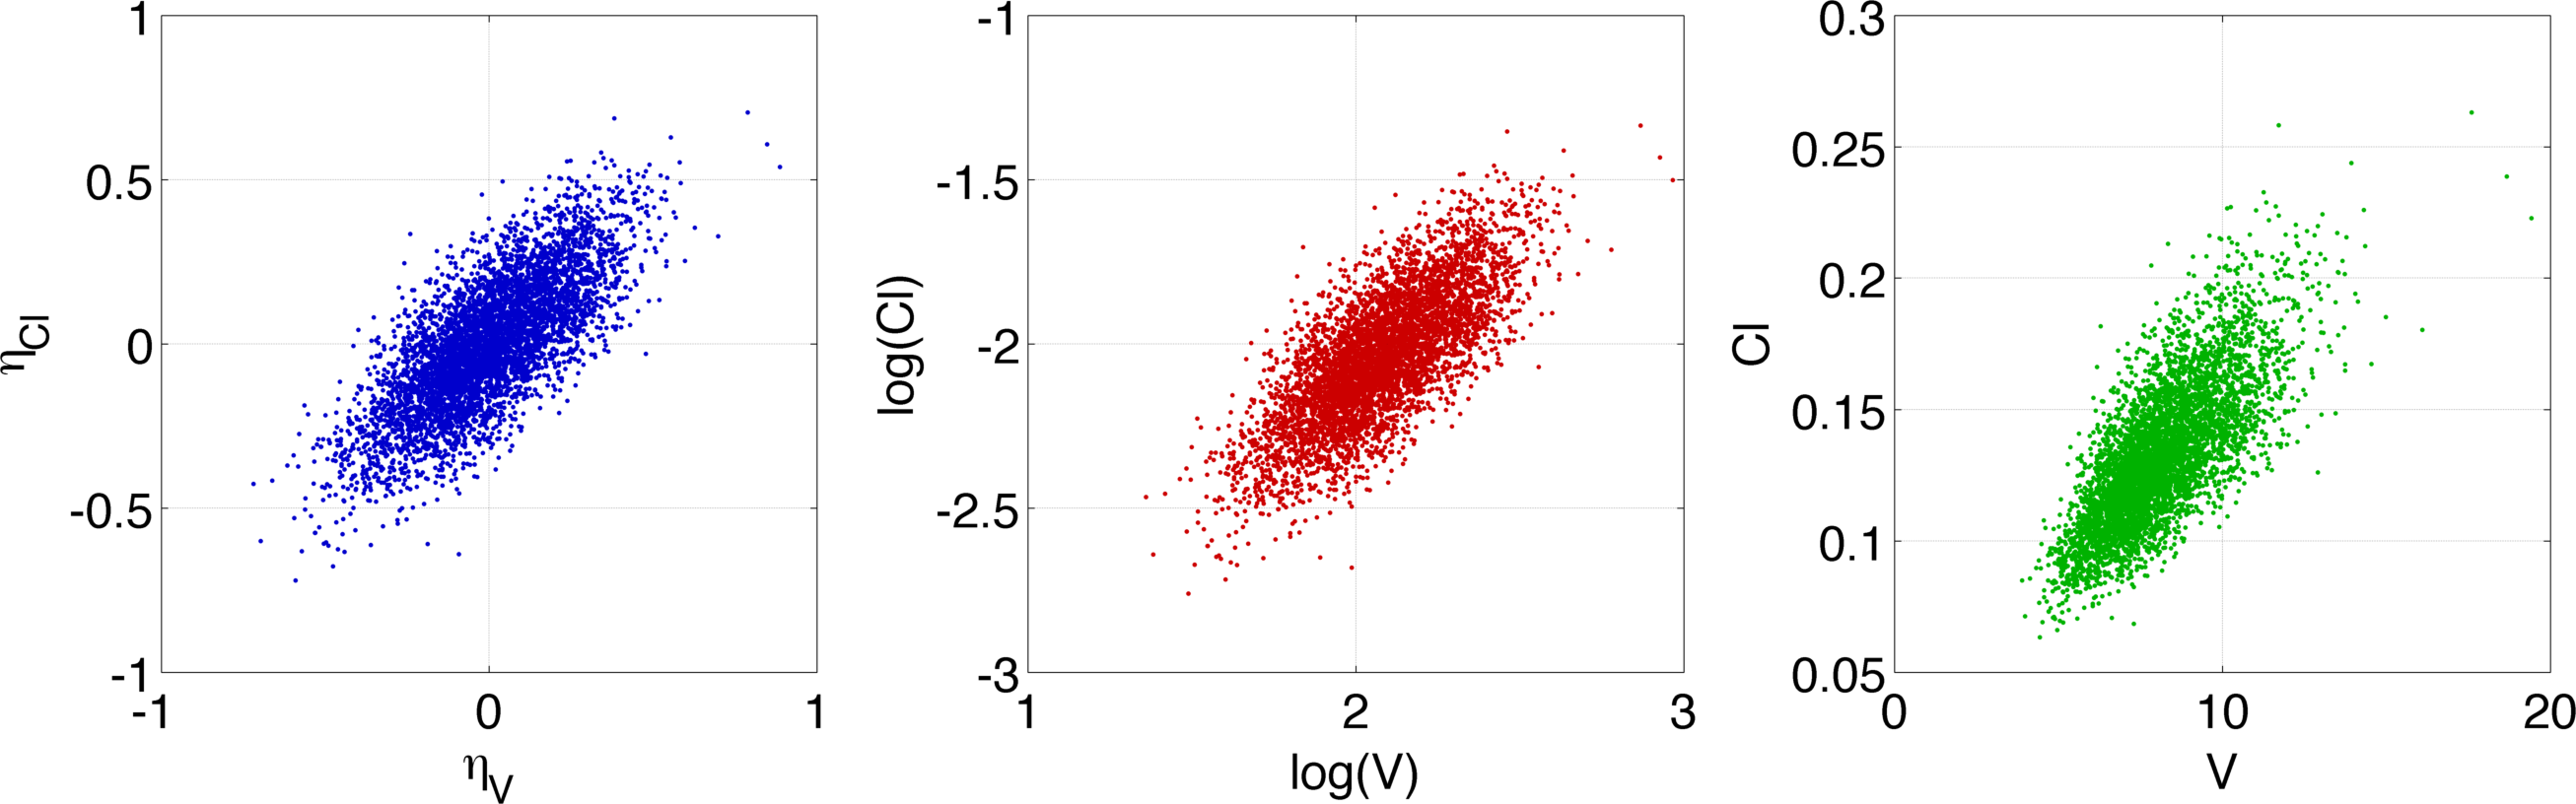
\includegraphics[height=45mm]{correlationsNoCovars}
%%\caption{Correlation of random effects $\eta_V$, $\eta_{CL}$ (blue), transformed parameters $\log(V)$ and $\log(CL)$ (red) and actual parameters  $V$ and $CL$ (green) is equal in the case without covariates. Values used: $V_{pop}=8, \omega_V=0.2, CL_{pop}=0.13,  \omega_{CL}=0.2$.}
%%\label{fig:correlationEtasLogedParams1}
%%\end{figure}
%%\newline
%%Now, we consider that both parameters depend on a continuous normally distributed covariate, e.g. the $Weight$,
%%\begin{align*}
%%& \eta_{V} \sim \mathcal{N}(0,\omega_V); \quad \log( V ) = \log( V_{pop} ) + \beta_{V} \log\Big(\frac{W}{70}\Big) + \eta_{V}  \\
%%& \eta_{CL} \sim \mathcal{N}(0,\omega_{CL}); \quad \log( CL ) = \log( CL_{pop} ) + \beta_{CL} \log\Big(\frac{W}{70}\Big) + \eta_{CL}
%%\end{align*}
%%then the correlation between the transformed parameters is higher then that of the random effects and increases proportionally to $corr(\eta_{V}, \eta_{CL})$, see Figure \ref{fig:correlationEtasLogedParams2}.
%%\begin{figure}[h!]
%%\centering
%% 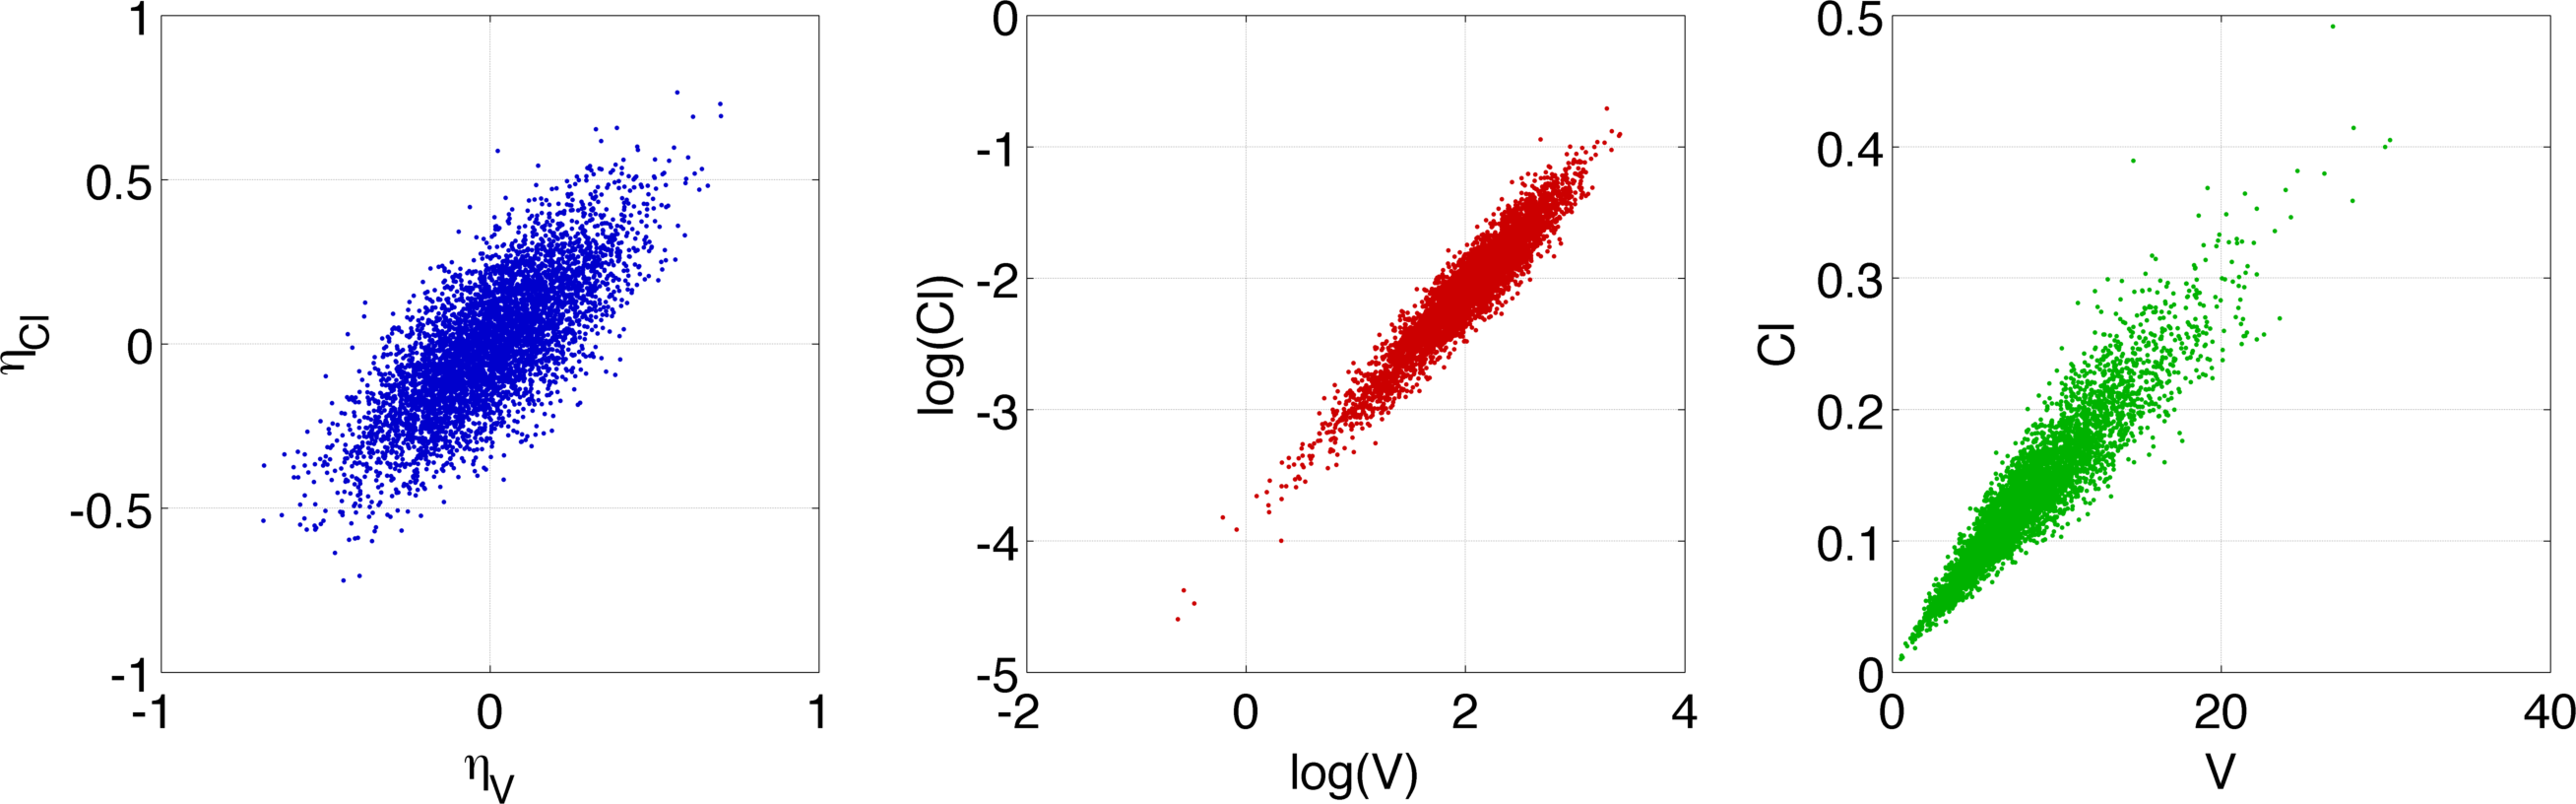
\includegraphics[height=45mm]{correlationsWithCovars}
%%\caption{The correlation between both the transformed parameters (red) and actual parameters (green) is higher then that of the random effects (blue) (and is equal 0.933, 0.948 and 0.750, respectively, for $n=10^8$). Values used as before with $\beta_V=2, \beta_{CL}= 1.75$.}
%%\label{fig:correlationEtasLogedParams2}
%%\end{figure}
%%\newline
%%The consequence of this discussion is that the correlation structure of random effects, as defined in PharmML, translates only in special cases to the correlation between parameters.
%%%This underlines the importance of the fact that we define in PharmML the relationship between random effects and not parameters.


%%%%%%%%%%%%%%%%%%%%%%%%%%%%%%%%%%%%%%%%%%%%%%%%%%%%%%%%%%%%%%%%%
\subsection{Equivalent representations of the parameter model}
Every parameter model represented in the Type 3 format discussed before has at least three mathematically equivalent representation forms,
which will be presented and discussed in terms of advantages and disadvantages in the following. It is important to understand these different
representation forms, as they explain the different forms of notation used in different software tools. Here, we concentrate on NONMEM and MONOLIX only.

%%%%%%%%%%%%%%%%%%%%%%%%%%%%%%%%%%%%%%%%%%%%%%%%%%%%%%%%%%%%%%%%%
% Log-Normal distributed
%%%%%%%%%%%%%%%%%%%%%%%%%%%%%%%%%%%%%%%%%%%%%%%%%%%%%%%%%%%%%%%%%

\subsubsection{Log-Normal distributed}
For a \textbf{log-normal} distributed parameter, e.g. $V$, the equivalent representations read
\begin{align*}
&(1) \eta_{i,V} \sim \mathcal{N}(0,\omega_V); \quad V_i= V_{pop} \; e^{\eta_{i,V}}   \\
&(2) \eta_{i,V} \sim \mathcal{N}(0,\omega_V); \quad \log( V_i ) = \log( V_{pop} ) + \eta_{i,V}  \\
&(3) \log( V_i ) \sim \mathcal{N}\big( \log( V_{pop} ),\omega_V\big)
\end{align*}
for a typical value $V_{pop}$ and standard deviation $\omega_V$ as described in \cite{LavielleBook:2014}.\\
The typical NMTRAN code for a log-normally distributed parameter is (\cite{Smith:2012aa})
\begin{lstlisting}
	GRPV=THETA(1)
	V=GRPV*EXP(ETA(1))
\end{lstlisting}
and in MLXTRAN (\cite{MonolixOverview:2012})
\begin{lstlisting}
	# as explicit equation
	eta_V ~ normal(0, omega_V)
	V = V_pop*exp(eta_V)

	# or using short notation
	V = {distribution=lognormal, typical=V_pop, sd=omega_V}
\end{lstlisting}

\begin{figure}[htbp]
\centering
 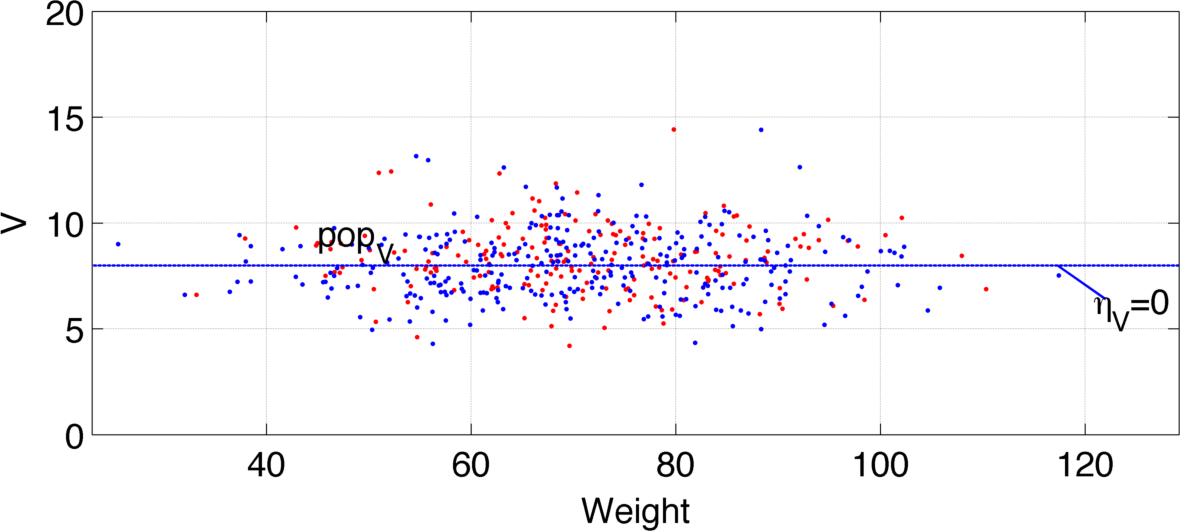
\includegraphics[width=100mm]{pics/paramCovModel_V}
\caption{Log-normally distributed 'V' with $V_{pop}=8$ and $\omega_V=0.2$}
\label{fig:parameterCovModel0}
\end{figure}


%%%%%%%%%%%%%%%%%%%%%%%%%%%%%%%%%%%%%%%%%%%%%%%%%%%%%%%%%%%%%%%%%
% Log-Normal distributed with a continuous covariate
%%%%%%%%%%%%%%%%%%%%%%%%%%%%%%%%%%%%%%%%%%%%%%%%%%%%%%%%%%%%%%%%%

\subsubsection{Log-Normal distributed with a continuous covariate}
For a \textbf{log-normal} distributed parameter, e.g. $V$, with body weight, $W$, as covariate the equivalent representations read
\begin{align*}
& (1) \quad \eta_{i,V} \sim \mathcal{N}(0,\omega_V); \quad V_i= V_{pop} \; \big(\frac{W_i}{70}\big)^\beta \; e^{\eta_{i,V}}   \\
&(2) \quad \eta_{i,V} \sim \mathcal{N}(0,\omega_V); \quad \log( V_i ) = \log( V_{pop} ) + \beta \log\big(\frac{W_i}{70}\big) + \eta_{i,V}  \\
&(3) \quad \log( V_i ) \sim \mathcal{N}\big( \log( V_{pop} )+ \beta\log\Big(\frac{W_i}{70}\Big),\omega_V\big)
\end{align*}
The typical NMTRAN code for a log-normally distributed parameter with weight as covariate is
\begin{lstlisting}
	GRPV=THETA(1)*(WT/70)**THETA(2)
	V=GRPV*EXP(ETA(1))
\end{lstlisting}
and in MLXTRAN
\begin{lstlisting}
	# as explicit equation
	V_pop = V_pop*(weight/70)^beta_V
	eta_V ~ normal(0, omega_V)	
	V = V_pop*exp(eta_V)

	# or using short notation
	V = {distribution=lognormal, typical=V_pop, covariate=lw70, coefficient=beta_V, sd=omega_V}
\end{lstlisting}
with $lw70 \equiv \log(W/70)$.

\begin{figure}[htbp]
\centering
 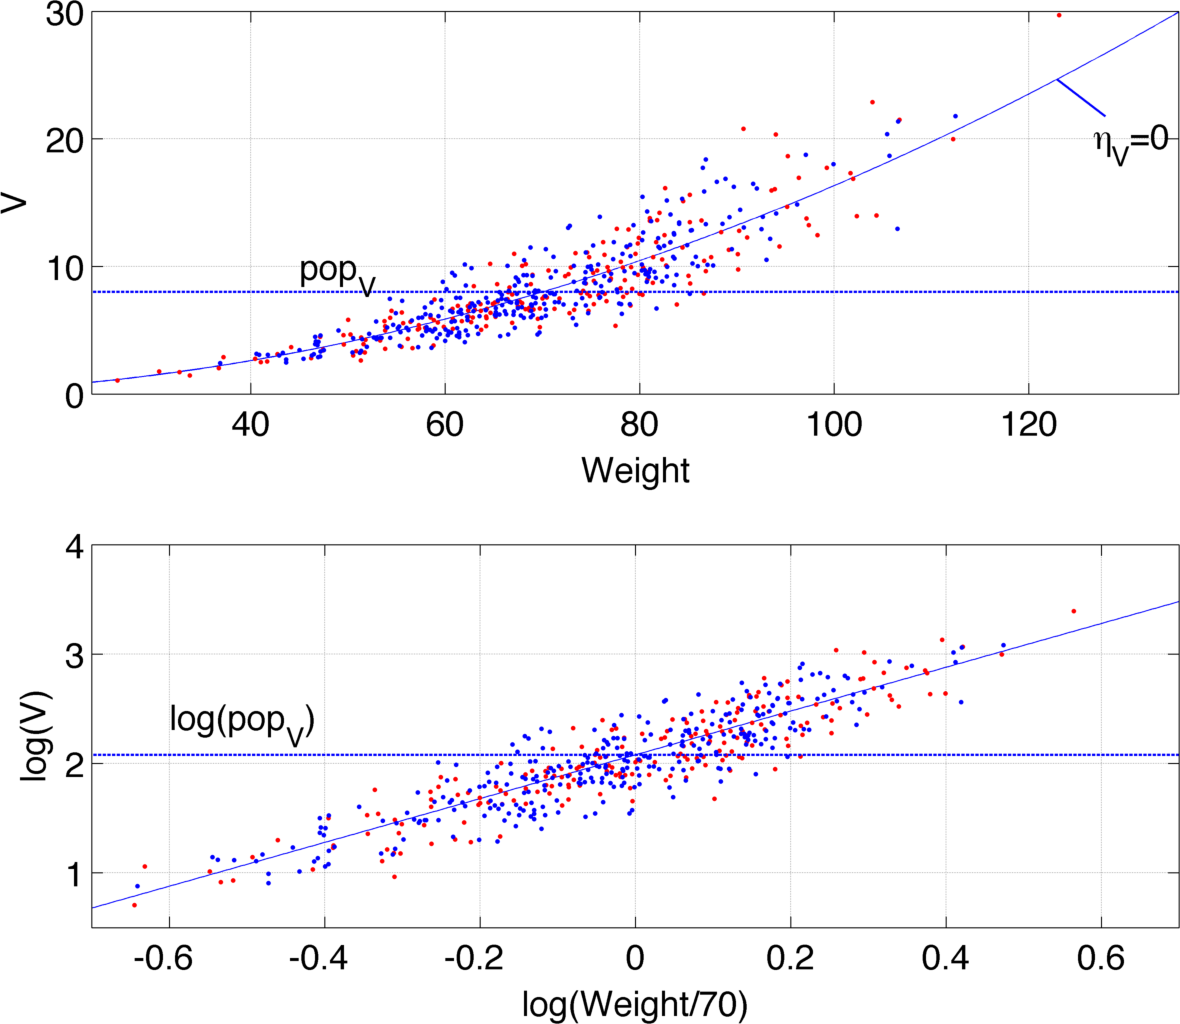
\includegraphics[width=100mm]{pics/paramCovModel_VlogV}
\caption{Log-normally distributed 'V' with 'Weight' as covariates.}
\label{fig:parameterCovModel1}
\end{figure}


%%%%%%%%%%%%%%%%%%%%%%%%%%%%%%%%%%%%%%%%%%%%%%%%%%%%%%%%%%%%%%%%%
% Logit-Normal distributed
%%%%%%%%%%%%%%%%%%%%%%%%%%%%%%%%%%%%%%%%%%%%%%%%%%%%%%%%%%%%%%%%%

\subsubsection{Logit-Normal distributed}
For a \textbf{logit-normal} distributed parameter, e.g. $Imax$, the equivalent representations read
\begin{align*}
&(1) \quad \eta_{i,Imax} \sim \mathcal{N}(0,\omega); \quad  Imax_i= \frac{\bigg[\frac{ Imax_{pop}}{1- Imax_{pop}} \; e^{\eta_{i, Imax}} \bigg]}{ 1+  \bigg[\frac{ Imax_{pop}}{1- Imax_{pop}} \; e^{\eta_{i, Imax}} \bigg]}   \\
&(2) \quad  \eta_{i,Imax} \sim \mathcal{N}(0,\omega); \quad \mbox{logit}(  Imax_i ) = \mbox{logit}(  Imax_{pop} ) + \eta_{i, Imax}  \\
&(3) \quad  \mbox{logit}(  Imax_i ) \sim \mathcal{N}\big( \mbox{logit}( Imax_{pop} ),\omega\big)
\end{align*}
Equation (1) can be rewritten using '$logit$' as follows
\begin{align*}
& Imax_i= \frac{\exp\big(logit(Imax_{pop})  + \eta_{i,Imax} \big)}{ 1+ \exp\big(logit(Imax_{pop}) + \eta_{i,Imax} \big)}  \\
& \Leftrightarrow  Imax_i= \frac{1}{ 1+ \exp\big(- logit(Imax_{pop}) - \eta_{i,Imax} \big)}
\end{align*}\newline
The last form is used for a typical NMTRAN implementation of a logit-normally distributed parameter
\begin{lstlisting}
	LGTIMAX=LOG(POP_IMAX/(1-POP_IMAX)) + ETA(IMAX)
	IMAX=1/(1+EXP(-LGTIMAX))
\end{lstlisting}
and in MLXTRAN
\begin{lstlisting}
	# as explicit equation
	eta_Imax ~ normal(0, omega_Imax)
	logitImaxi = log(pop_Imax/(1-pop_Imax)) + eta_Imax
	Imaxi = 1/(1 + exp(-logitImaxi))

	# or using short notation
	Imax = {distribution=logitnormal, typical=Imax_pop, sd=omega_Imax}
\end{lstlisting}


%%%%%%%%%%%%%%%%%%%%%%%%%%%%%%%%%%%%%%%%%%%%%%%%%%%%%%%%%%%%%%%%%
% Logit-Normal distributed with a continuous covariate
%%%%%%%%%%%%%%%%%%%%%%%%%%%%%%%%%%%%%%%%%%%%%%%%%%%%%%%%%%%%%%%%%

\subsubsection{Logit-Normal distributed with a continuous covariate}
For a \textbf{logit-normal} distributed parameter with \textit{Weight} as \textbf{covariate} we have
\begin{align*}
&(1)\quad \eta_{i,Imax} \sim \mathcal{N}(0,\omega); \quad Imax_i= \frac{\bigg[\frac{Imax_{pop}}{1-Imax_{pop}} \; \big(\frac{W_i}{70}\big)^\beta \; e^{\eta_{i,Imax}} \bigg]}{ 1+  \bigg[\frac{Imax_{pop}}{1-Imax_{pop}} \; \big(\frac{W_i}{70}\big)^\beta \; e^{\eta_{i,Imax}} \bigg]}
\end{align*}
\begin{align*}
&(2)\quad \eta_{i,Imax} \sim \mathcal{N}(0,\omega); \quad \mbox{logit}( Imax_i ) = \mbox{logit}( Imax_{pop} ) + \beta \log\bigg(\frac{W_i}{70}\bigg) + \eta_{i,Imax}  \\
&(3)\quad \mbox{logit}(  Imax_i ) \sim \mathcal{N}\big( \mbox{logit}( Imax_{pop}) + \beta\log\Big(\frac{W_i}{70}\Big),\omega\big)
\end{align*}
The first equation can be rewritten as follows
\begin{align*}
& Imax_i= \frac{\exp\big(logit(Imax_{pop}) + \beta \log\big(\frac{W_i}{70}\big) + \eta_{i,Imax} \big)}{ 1+ \exp\big(logit(Imax_{pop}) + \beta \log\big(\frac{W_i}{70}\big) + \eta_{i,Imax} \big)}  \\
& \Leftrightarrow Imax_i= \frac{1}{ 1+ \exp\big(- logit(Imax_{pop}) - \beta \log\big(\frac{W_i}{70}\big) - \eta_{i,Imax} \big)}
\end{align*}\newline
The last form is used for a typical NMTRAN implementation of a logit-normally distributed parameter with covariate
\begin{lstlisting}
	LGTIMAX=LOG(POP_IMAX/(1-POP_IMAX)) + BETA*LOG(WT/70) + ETA(IMAX)
	IMAX=1/(1+EXP(-LGTIMAX))
\end{lstlisting}
and in MLXTRAN
\begin{lstlisting}
	# as explicit equation
	eta_Imax ~ normal(0, omega_Imax)
	logitImaxi = log(pop_Imax/(1-pop_Imax)) + beta*lw70 + eta_Imax
	Imaxi = 1/(1 + exp(-logitImaxi))

	# or using short notation
	Imax =	{distribution=lognormal, typical=Imax_pop, covariate=lw70, coefficient=beta_Imax, sd=omega_Imax}
\end{lstlisting}

\begin{figure}[htbp]
\centering
 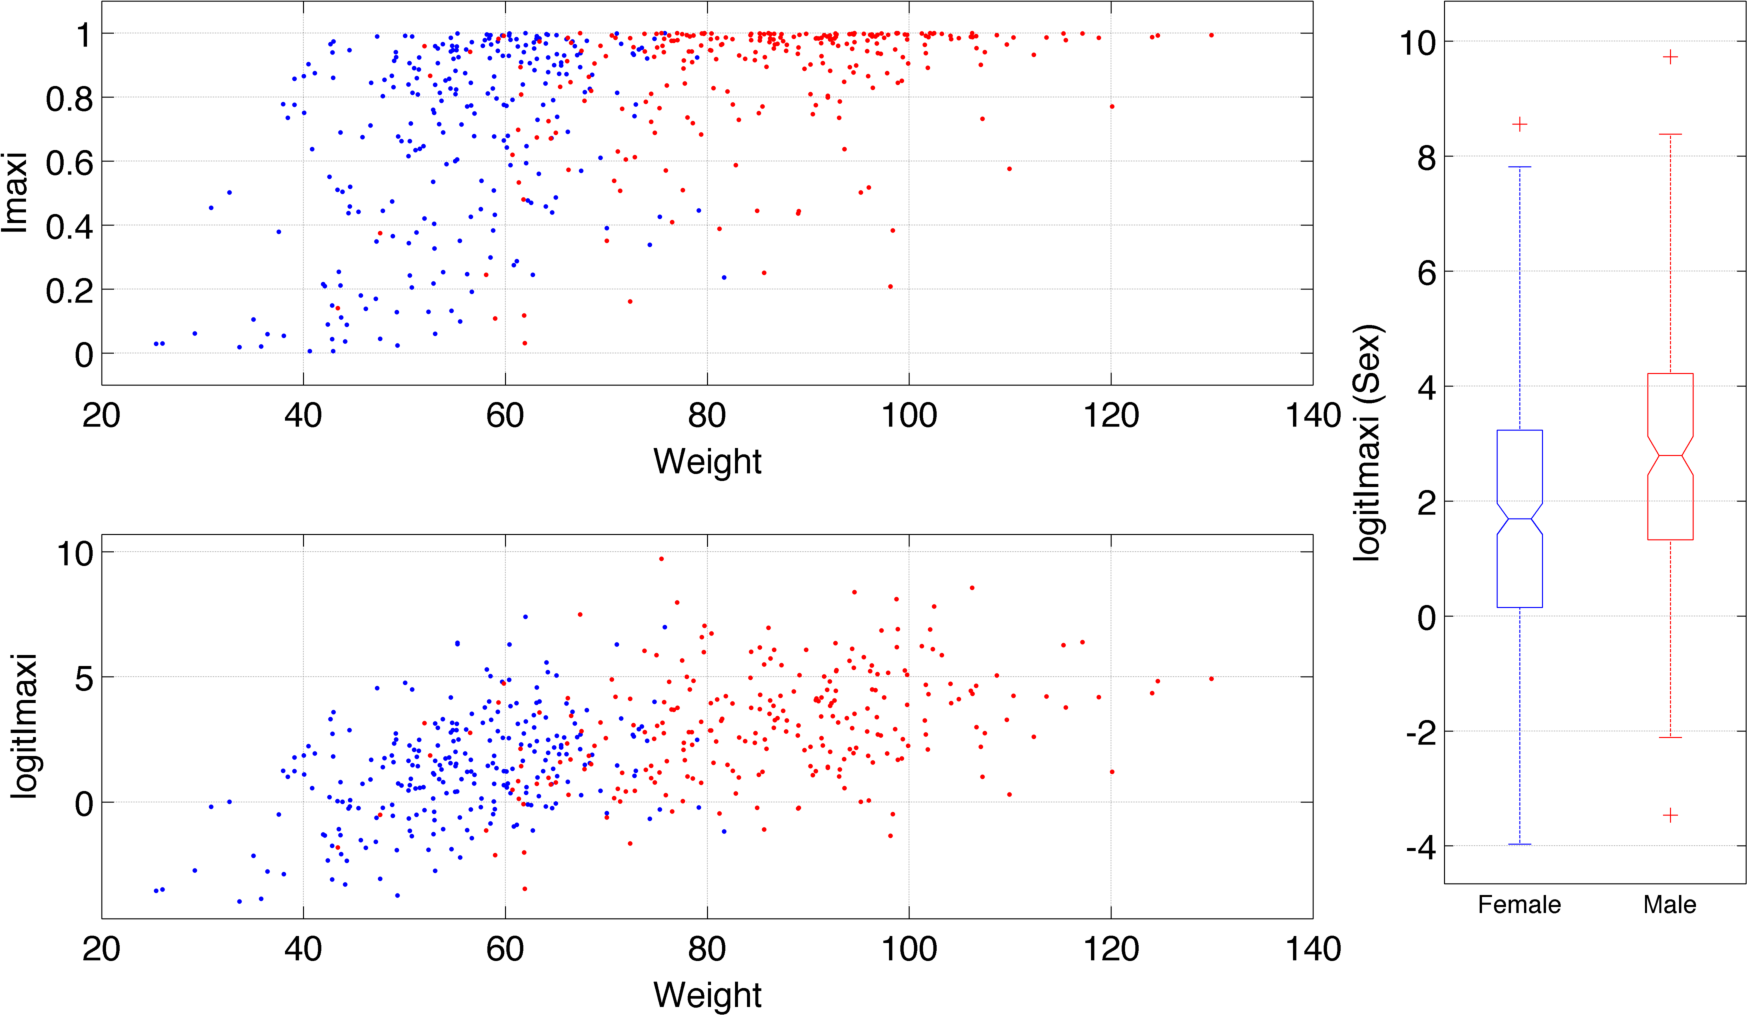
\includegraphics[width=100mm]{pics/paramCovModel_ImaxlogImax_Weight}
\caption{Logit-normally distributed 'Imax' with 'Weight' as covariate.}
\label{fig:parameterCovModel3}
\end{figure}


%%%%%%%%%%%%%%%%%%%%%%%%%%%%%%%%%%%%%%%%%%%%%%%%%%%%%%%%%%%%%%%%%%
%% Logit-Normal distributed with a categorical covariate
%%%%%%%%%%%%%%%%%%%%%%%%%%%%%%%%%%%%%%%%%%%%%%%%%%%%%%%%%%%%%%%%%%
%
%\subsubsection{Logit-Normal distributed with a categorical covariate}
%For a \textbf{logit-normal} distributed parameter with \textit{Sex} as \textbf{covariate} we have
%\begin{align*}
%&(1)\quad \eta_i \sim \mathcal{N}(0,\omega); \quad Imax_i= \frac{\bigg[\frac{Imax_{pop}}{1-Imax_{pop}} \; e^{\beta_{Imax_i} 1_{Sex_i=F}} \; e^{\eta_{i,Imax}} \bigg]}{ 1+  \bigg[\frac{Imax_{pop}}{1-Imax_{pop}} \; e^{\beta_{Imax_i} 1_{Sex_i=F}} \; e^{\eta_{i,Imax}} \bigg]}  \\
%&(2)\quad \eta_i \sim \mathcal{N}(0,\omega); \quad \mbox{logit}( Imax_i ) = \mbox{logit}( Imax_{pop} ) + \beta_{Imax_i} 1_{Sex_i=F} + \eta_{i,Imax}  \\
%&(3)\quad \mbox{logit}(  Imax_i ) \sim \mathcal{N}\big( \mbox{logit}( Imax_{pop}) + \beta_{Imax_i} 1_{Sex_i=F},\omega\big)
%\end{align*}
%The first equation can be rewritten as follows
%\begin{align*}
%& Imax_i= \frac{\exp\big(logit(Imax_{pop}) + \beta_{Imax_i} 1_{Sex_i=F} + \eta_{i,Imax} \big)}{ 1+ \exp\big(logit(Imax_{pop}) + \beta_{Imax_i} 1_{Sex_i=F} + \eta_{i,Imax} \big)}  \\
%& \Leftrightarrow Imax_i= \frac{1}{ 1+ \exp\big(- logit(Imax_{pop}) - \beta_{Imax_i} 1_{Sex_i=F} - \eta_{i,Imax} \big)}
%\end{align*}\newline
%The last form is used for a typical implementation of a logit-normally distributed parameter with covariate:\\
%in NMTRAN
%\begin{lstlisting}
%LGTIMAX=LOG(POP_IMAX/(1-POP_IMAX)) + BETA*SEX + ETA(IMAX)
%IMAX=1/(1+EXP(-LGTIMAX))
%\end{lstlisting}
%and in MLXTRAN
%\begin{lstlisting}
%# as explicit equation
%eta_Imax ~ normal(0, omega_Imax)
%logitImaxi = log(pop_Imax/(1-pop_Imax)) + beta*Sex + eta_Imax
%Imaxi = 1/(1 + exp(-logitImaxi))
%
%# or using short notation
%Imax =	{distribution=lognormal, typical=Imax_pop, covariate=Sex, coefficient=beta_Imax, sd=omega_Imax}
%\end{lstlisting}
%
%
%\begin{figure}[h!]
%\centering
% 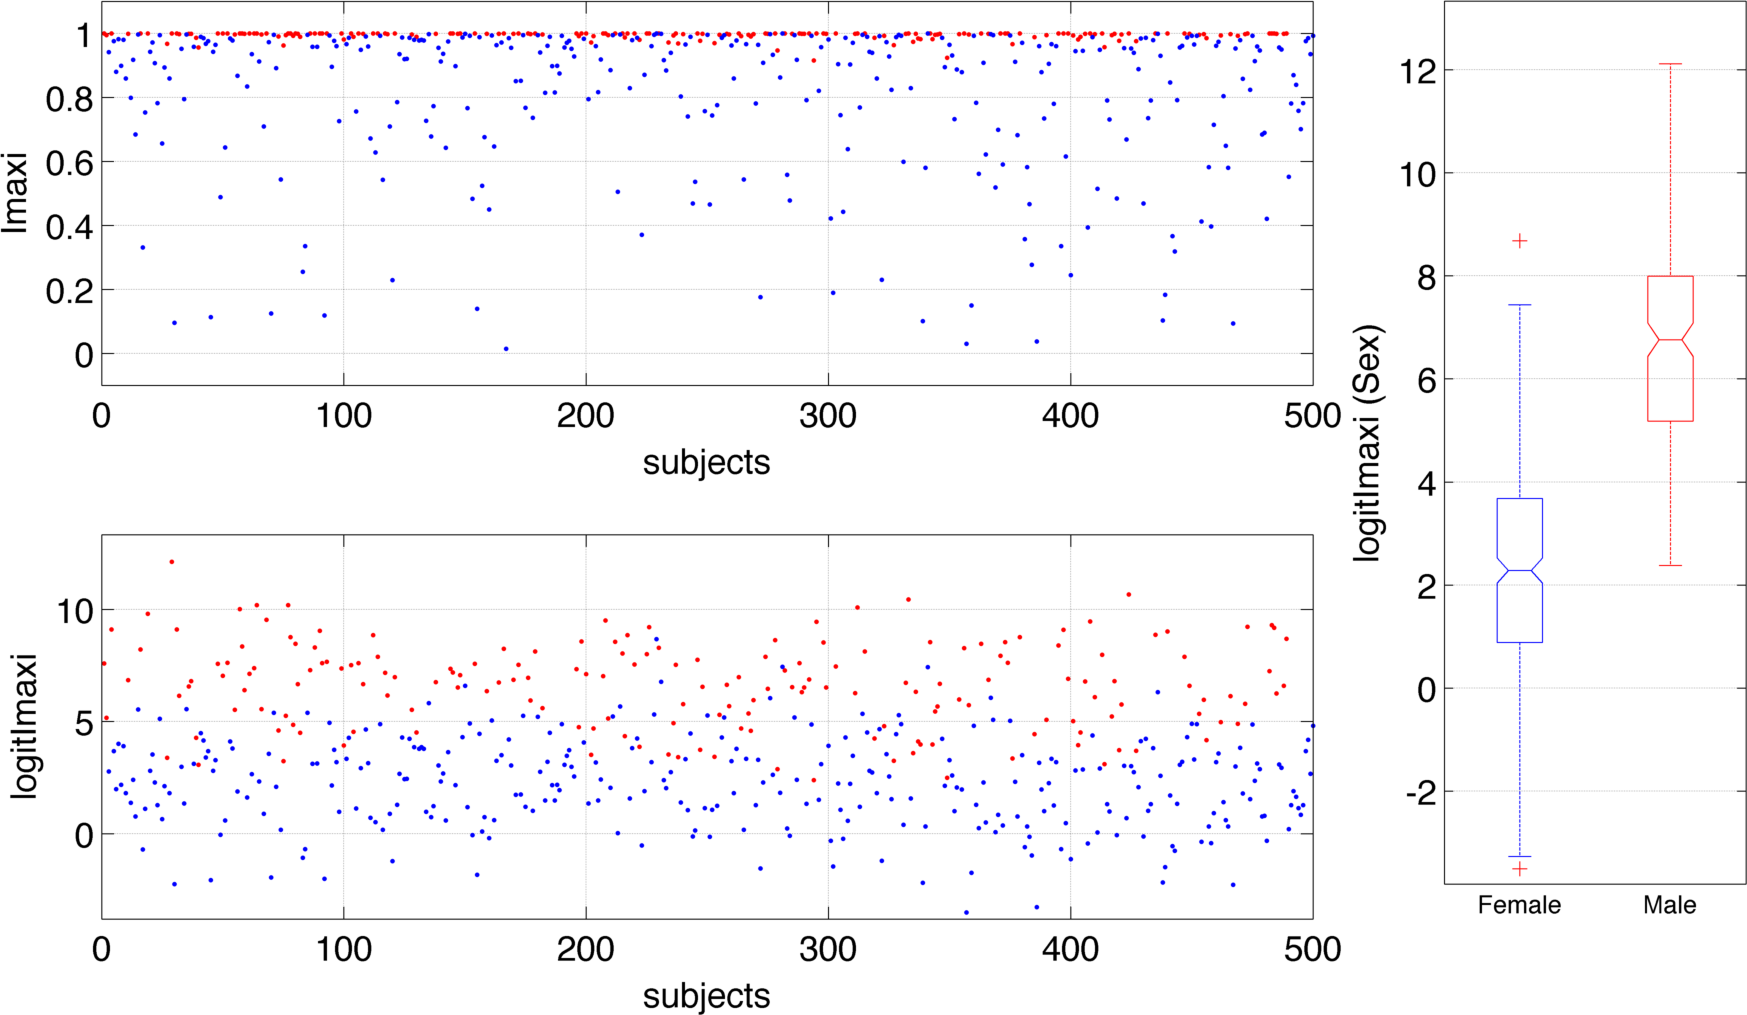
\includegraphics[width=100mm]{paramCovModel_ImaxlogImax_Sex}
%\caption{Logit-normally distributed 'Imax' with 'Sex' as a categorical covariate.}
%\label{fig:parameterCovModel4}
%\end{figure}


%%%%%%%%%%%%%%%%%%%%%%%%%%%%%%%%%%%%%%%%%%%%%%%%%%%%%%%%%%%%%%%%%
% Log-Normal distributed with complex variability structure
%%%%%%%%%%%%%%%%%%%%%%%%%%%%%%%%%%%%%%%%%%%%%%%%%%%%%%%%%%%%%%%%%

\subsubsection{Log-Normal distributed with complex variability structure}
\label{subsec:logIOVCovariate}
In this example we consider representations of type (1) and (2) only. A typical parameter model with a continuous covariate, $W$, for three levels of variability e.g. \{centre, subject, occasion\} (this will be explained in detail in next section), see Figure \ref{tree_IOV1}, reads as follows
\begin{align*}
&(1)\quad V_{lik} = V_{pop} \; \big(\frac{W_i}{70}\big)^\beta \; e^{\eta_{l,V}^{(-1)}} \; e^{\eta_{li,V}^{(0)}} \; e^{\eta_{lik,V}^{(+1)}}   \\
&(2)\quad \log(V_{lik}) = \log(V_{pop}) + \beta\log\Big(\frac{W_i}{70}\Big) + \eta_{l,V}^{(-1)} + \eta_{li,V}^{(0)} + \eta_{lik,V}^{(+1)}
\end{align*}
with
\begin{align*}
 & \eta_l^{(-1)} \sim \mathcal{N}\big(0,\Omega^{(-1)}\big), \quad \eta_{li}^{(0)} \sim \mathcal{N}\big(0,\Omega^{(0)}\big),
\quad \eta_{lik}^{(+1)} \sim \mathcal{N}\big(0,\Omega^{(+1)}\big)
\end{align*}
with $l$ -- centre index, $i$ -- subject index, $k$ -- occasion index.


%%%%%%%%%%%%%%%%%%%%%%%%%%%%%%%%%%%%%%%%%%%%%%%%%%%%%%%%%%%%%%%%%
% Discussion
%%%%%%%%%%%%%%%%%%%%%%%%%%%%%%%%%%%%%%%%%%%%%%%%%%%%%%%%%%%%%%%%%
%
%\subsection{Discussion}
%Currently, \pharmml supports the version (2) of the parameter model. Consider the parameter model from last example
%which with some additional annotation reads as follows
%\begin{align*}
%& \underbrace{\log(V_{lik})}_{\text{\parbox{2cm}{\centering transformed\\[-4pt] individual value}}} = \underbrace{\log(V_{pop})}_{\text{\parbox{2cm}{\centering transformed\\[-4pt] typical value}}} + \underbrace{\beta\log\Big(\frac{W_i}{70}\Big)}_{\text{covariate model}}
%+ \underbrace{\eta_{l,V}^{(1)}}_{\text{\parbox{2cm}{\centering inter-centre\\[-4pt]  variability}}}
%+ \underbrace{\eta_{li,V}^{(0)}}_{\text{\parbox{2cm}{\centering inter-individual\\[-4pt] within centre \\[-4pt]  variability}}}
%+ \underbrace{\eta_{lik,V}^{(-1)}}_{\text{\parbox{2.5cm}{\centering inter-occasion\\[-4pt] within individual \\[-4pt] within centre \\[-4pt] variability}}}
%\end{align*}
%This formula, linear for the transformed parameter, has the following \textbf{advantages}
%\begin{itemize}
%\item
%it has an additive structure allowing for easy interpretation and implementation of its components, i.e.
%\begin{itemize}
%\item
%typical/population value of the parameter
%\item
%covariate model
%\item
%any level of random effects
%\end{itemize}
%\item
%it covers the majority of models relevant for daily practice
%\end{itemize}
%The \textbf{disadvantage} is that it doesn't cover parameter models which cannot be represented in the linear form for the transformed parameter, e.g. the models proposed by \cite{Keizer:2011aa}. This issue has been recognised early on and discussed in the consortium. This class of models is being considered for a subsequent specification of \pharmml.


%
%\paragraph{Discussion}
%Consider for example equation (2) for a parameter with a continuous covariate, $W$, with three levels of variability e.g. \{country,subject, occasion\} from the last example. With some additional annotation it reads then
%\begin{align*}
%& \underbrace{\log(V_{lik})}_{\parbox{2cm}{\centering transformed\\[-4pt] individual\\[-4pt] value}} = \underbrace{\log(V_{pop})}_{\parbox{1.5cm}{\centering transformed\\[-4pt] typical\\[-4pt] value}}
%+ \underbrace{\beta\log\Big(\frac{W_i}{70}\Big)}_{\parbox{2cm}{\centering covariate\\[-4pt] model}}
%+ \underbrace{\eta_{l,V}^{(1)}}_{\parbox{2cm}{\centering inter-centre\\[-4pt]  variability}}
%+ \underbrace{\eta_{li,V}^{(0)}}_{\parbox{2.25cm}{\centering inter-centre-\\[-4pt] individual\\[-4pt]  variability}}
%+ \underbrace{\eta_{lik,V}^{(-1)}}_{\parbox{3cm}{\centering inter-centre-\\[-4pt] individual-occasion\\[-4pt] variability}}
%\end{align*}
%
%This formulation, linear for the transformed parameter, has the following advantages
%\begin{itemize}
%\item
%it has an additive structure allowing for easy interpretation and implementation of its components, i.e.
%\begin{itemize}
%\item
%typical/population value of the parameter
%\item
%covariate model
%\item
%inter-individual variability random effects
%\item
%higher levels of variability
%\end{itemize}
%\item
%it covers the majority of models relevant for daily practice
%\end{itemize}
%More complex models will be supported in an upcoming specification.
%
